% ============================================================
% Day 13 - Model Comparison & Feature Engineering
% Databricks 14-Day AI Challenge
% Databricks Theme LaTeX Beamer Presentation
% ============================================================

\documentclass[aspectratio=169]{beamer}

% ============================================================
% Packages
% ============================================================
\usepackage{tikz}
\usepackage{graphicx}
\usepackage{hyperref}
\usepackage{xcolor}
\usepackage{amsmath}
\usepackage{amssymb}
\usepackage{booktabs}
\usepackage{listings}
\usepackage{fontspec}
\usepackage{array}
\usepackage{tabularx}
\usepackage{multirow}
\usepackage{colortbl}

\usetikzlibrary{shapes.geometric, arrows.meta, positioning, calc, fit, backgrounds}

% ============================================================
% Databricks Color Palette
% ============================================================
\definecolor{databricksBlue}{RGB}{41, 49, 66}
\definecolor{databricksRed}{RGB}{220, 53, 69}
\definecolor{databricksYellow}{RGB}{255, 193, 7}
\definecolor{databricksGreen}{RGB}{76, 175, 80}
\definecolor{databricksGray}{RGB}{128, 128, 128}
\definecolor{databricksLightGray}{RGB}{245, 245, 245}
\definecolor{databricksWhite}{RGB}{255, 255, 255}
\definecolor{databricksOrange}{RGB}{255, 140, 0}
\definecolor{databricksPurple}{RGB}{156, 39, 176}

% ============================================================
% Beamer Theme Configuration
% ============================================================
\usetheme{default}
\usecolortheme{default}

% Set colors
\setbeamercolor{structure}{fg=databricksBlue}
\setbeamercolor{title}{fg=databricksWhite}
\setbeamercolor{subtitle}{fg=databricksLightGray}
\setbeamercolor{author}{fg=databricksWhite}
\setbeamercolor{date}{fg=databricksLightGray}
\setbeamercolor{frametitle}{fg=databricksWhite, bg=databricksBlue}
\setbeamercolor{normal text}{fg=databricksBlue}
\setbeamercolor{block title}{fg=databricksWhite, bg=databricksBlue}
\setbeamercolor{block body}{bg=databricksLightGray}
\setbeamercolor{itemize item}{fg=databricksBlue}
\setbeamercolor{itemize subitem}{fg=databricksRed}

% Set fonts
\setbeamerfont{title}{size=\Huge, series=\bfseries}
\setbeamerfont{subtitle}{size=\large}
\setbeamerfont{frametitle}{size=\Large, series=\bfseries}

% Remove navigation symbols
\setbeamertemplate{navigation symbols}{}

% ============================================================
% Custom Footer
% ============================================================
\setbeamertemplate{footline}{
    \leavevmode%
    \hbox{%
        \begin{beamercolorbox}[wd=.333333\paperwidth,ht=2.5ex,dp=1ex,left]{author in head/foot}%
            \usebeamerfont{author in head/foot}\hspace*{2ex}%
            \href{https://easy-ai-labs.lovable.app/}{\textcolor{databricksBlue}{Easy AI Labs}}
        \end{beamercolorbox}%
        \begin{beamercolorbox}[wd=.333333\paperwidth,ht=2.5ex,dp=1ex,center]{title in head/foot}%
            \usebeamerfont{title in head/foot}%
            \href{https://www.linkedin.com/in/yashkavaiya}{\textcolor{databricksBlue}{Yash Kavaiya}}
        \end{beamercolorbox}%
        \begin{beamercolorbox}[wd=.333333\paperwidth,ht=2.5ex,dp=1ex,right]{date in head/foot}%
            \usebeamerfont{date in head/foot}%
            \href{https://www.linkedin.com/company/genai-guru}{\textcolor{databricksBlue}{Gen AI Guru}}\hspace*{2ex}
            \textcolor{databricksGray}{\insertframenumber{} / \inserttotalframenumber}\hspace*{2ex}
        \end{beamercolorbox}%
    }%
    \vskip0pt%
}

% ============================================================
% Custom Header
% ============================================================
\setbeamertemplate{frametitle}{
    \nointerlineskip
    \begin{beamercolorbox}[wd=\paperwidth,ht=2.5ex,dp=1ex]{frametitle}
        \hspace*{1ex}\insertframetitle
    \end{beamercolorbox}
}

% ============================================================
% Code Listing Style
% ============================================================
\lstdefinestyle{pythonstyle}{
    language=Python,
    basicstyle=\ttfamily\footnotesize,
    keywordstyle=\color{databricksBlue}\bfseries,
    stringstyle=\color{databricksGreen},
    commentstyle=\color{databricksGray}\itshape,
    numberstyle=\tiny\color{databricksGray},
    numbers=left,
    numbersep=5pt,
    breaklines=true,
    showstringspaces=false,
    frame=single,
    rulecolor=\color{databricksBlue},
    backgroundcolor=\color{databricksLightGray},
    tabsize=2
}
\lstset{style=pythonstyle}

% ============================================================
% Title Page Information
% ============================================================
\title{Day 13: Model Comparison \& Feature Engineering}
\subtitle{Databricks 14-Day AI Challenge}
\author{Yash Kavaiya}
\date{\today}

% ============================================================
% Document Begin
% ============================================================
\begin{document}

% ============================================================
% Title Slide
% ============================================================
{
\setbeamertemplate{footline}{}
\begin{frame}
\begin{tikzpicture}[remember picture, overlay]
    % Background
    \fill[databricksBlue] (current page.south west) rectangle (current page.north east);
    
    % Decorative elements
    \fill[databricksRed, opacity=0.3] (current page.north west) ++(0,-2) circle (3cm);
    \fill[databricksYellow, opacity=0.2] (current page.south east) ++(-1,1) circle (4cm);
    \fill[databricksGreen, opacity=0.2] (current page.east) ++(-2,0) circle (2cm);
    
    % Title content
    \node[anchor=center, text width=0.85\paperwidth, align=center] at (current page.center) {
        {\Huge\bfseries\textcolor{databricksWhite}{Day 13}}\\[0.3cm]
        {\LARGE\textcolor{databricksYellow}{Model Comparison \&}}\\[0.2cm]
        {\LARGE\textcolor{databricksYellow}{Feature Engineering}}\\[0.8cm]
        {\large\textcolor{databricksLightGray}{Databricks 14-Day AI Challenge}}\\[0.5cm]
        {\normalsize\textcolor{databricksWhite}{Yash Kavaiya}}
    };
    
    % Bottom decoration
    \fill[databricksYellow] (current page.south west) rectangle ++(0.5\paperwidth, 0.15);
    \fill[databricksRed] (current page.south west) ++(0.5\paperwidth,0) rectangle ++(0.5\paperwidth, 0.15);
\end{tikzpicture}
\end{frame}
}

% ============================================================
% Agenda Slide
% ============================================================
\begin{frame}{Agenda}
    \begin{columns}[T]
        \begin{column}{0.48\textwidth}
            \textcolor{databricksBlue}{$\bullet$} \textcolor{databricksBlue}{\textbf{Training Multiple Models}}
            \begin{itemize}
                \item[\textcolor{databricksRed}{$\triangleright$}] Why compare different algorithms?
                \item[\textcolor{databricksRed}{$\triangleright$}] Common regression models
            \end{itemize}
            \vspace{0.3cm}
            
            \textcolor{databricksBlue}{$\bullet$} \textcolor{databricksBlue}{\textbf{Hyperparameter Tuning}}
            \begin{itemize}
                \item[\textcolor{databricksRed}{$\triangleright$}] Parameters vs Hyperparameters
                \item[\textcolor{databricksRed}{$\triangleright$}] Tuning techniques
            \end{itemize}
            \vspace{0.3cm}
            
            \textcolor{databricksBlue}{$\bullet$} \textcolor{databricksBlue}{\textbf{Feature Importance}}
            \begin{itemize}
                \item[\textcolor{databricksRed}{$\triangleright$}] Methods to calculate importance
                \item[\textcolor{databricksRed}{$\triangleright$}] Interpretation and use cases
            \end{itemize}
        \end{column}
        
        \begin{column}{0.48\textwidth}
            \textcolor{databricksBlue}{$\bullet$} \textcolor{databricksBlue}{\textbf{Spark ML Pipelines}}
            \begin{itemize}
                \item[\textcolor{databricksRed}{$\triangleright$}] Pipeline components
                \item[\textcolor{databricksRed}{$\triangleright$}] Building reproducible workflows
            \end{itemize}
            \vspace{0.3cm}
            
            \textcolor{databricksBlue}{$\bullet$} \textcolor{databricksBlue}{\textbf{MLflow Integration}}
            \begin{itemize}
                \item[\textcolor{databricksRed}{$\triangleright$}] Experiment tracking
                \item[\textcolor{databricksRed}{$\triangleright$}] Model comparison
            \end{itemize}
            \vspace{0.3cm}
            
            \textcolor{databricksBlue}{$\bullet$} \textcolor{databricksBlue}{\textbf{Best Practices}}
            \begin{itemize}
                \item[\textcolor{databricksRed}{$\triangleright$}] Model selection guide
                \item[\textcolor{databricksRed}{$\triangleright$}] Production deployment
            \end{itemize}
        \end{column}
    \end{columns}
\end{frame}

% ============================================================
% Section: Introduction
% ============================================================
\begin{frame}{Introduction}
    \begin{block}{Model Comparison \& Feature Engineering}
        Critical steps in the machine learning lifecycle that determine production success.
    \end{block}
    
    \vspace{0.3cm}
    
    \begin{columns}[T]
        \begin{column}{0.48\textwidth}
            \textcolor{databricksBlue}{\textbf{What We'll Cover:}}
            \begin{itemize}
                \item[\textcolor{databricksBlue}{$\bullet$}] Training multiple regression models
                \item[\textcolor{databricksBlue}{$\bullet$}] Tracking experiments with MLflow
                \item[\textcolor{databricksBlue}{$\bullet$}] Building ML pipelines with Spark
                \item[\textcolor{databricksBlue}{$\bullet$}] Understanding feature importance
            \end{itemize}
        \end{column}
        
        \begin{column}{0.48\textwidth}
            \textcolor{databricksRed}{\textbf{Why It Matters:}}
            \begin{itemize}
                \item[\textcolor{databricksRed}{$\triangleright$}] Rarely deploy the first model
                \item[\textcolor{databricksRed}{$\triangleright$}] Systematic comparison needed
                \item[\textcolor{databricksRed}{$\triangleright$}] Better model = better business outcomes
            \end{itemize}
        \end{column}
    \end{columns}
\end{frame}

% ============================================================
% Section: Why Train Multiple Models
% ============================================================
\begin{frame}{Why Train Multiple Models?}
    \begin{block}{The "No Free Lunch" Theorem}
        No single algorithm works best for every problem — each has unique strengths!
    \end{block}
    
    \vspace{0.4cm}
    
    \begin{columns}[T]
        \begin{column}{0.5\textwidth}
            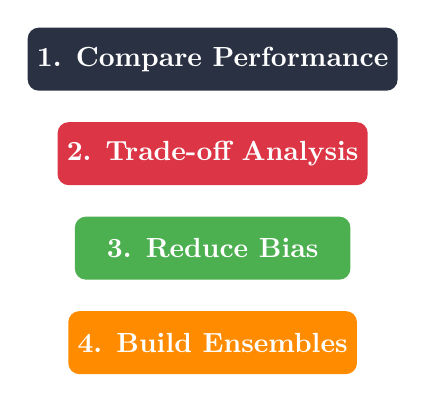
\begin{tikzpicture}
                \node[fill=databricksBlue, text=white, rounded corners, minimum width=3.5cm, minimum height=0.8cm] (c1) at (0,0) {\textbf{1. Compare Performance}};
                \node[fill=databricksRed, text=white, rounded corners, minimum width=3.5cm, minimum height=0.8cm] (c2) at (0,-1.2) {\textbf{2. Trade-off Analysis}};
                \node[fill=databricksGreen, text=white, rounded corners, minimum width=3.5cm, minimum height=0.8cm] (c3) at (0,-2.4) {\textbf{3. Reduce Bias}};
                \node[fill=databricksOrange, text=white, rounded corners, minimum width=3.5cm, minimum height=0.8cm] (c4) at (0,-3.6) {\textbf{4. Build Ensembles}};
            \end{tikzpicture}
        \end{column}
        
        \begin{column}{0.5\textwidth}
            \footnotesize
            \begin{itemize}
                \item[\textcolor{databricksBlue}{$\bullet$}] See which algorithm captures patterns best
                \vspace{0.2cm}
                \item[\textcolor{databricksRed}{$\bullet$}] Balance accuracy vs. interpretability
                \vspace{0.2cm}
                \item[\textcolor{databricksGreen}{$\bullet$}] Avoid single algorithm assumptions
                \vspace{0.2cm}
                \item[\textcolor{databricksOrange}{$\bullet$}] Combine models for better predictions
            \end{itemize}
        \end{column}
    \end{columns}
\end{frame}

% ============================================================
% Section: Common Regression Models
% ============================================================
\begin{frame}{Common Regression Models}
    \centering
    \small
    \begin{tabular}{>{\columncolor{databricksBlue}\color{white}}l c c c c}
        \toprule
        \textbf{Model} & \textbf{Type} & \textbf{Strengths} & \textbf{Weaknesses} & \textbf{Interpretability} \\
        \midrule
        \rowcolor{databricksLightGray}
        Linear Regression & Parametric & Fast, Simple & Linear assumption & \textcolor{databricksGreen}{High} \\
        Decision Tree & Non-parametric & Handles non-linearity & Prone to overfit & \textcolor{databricksYellow}{Medium} \\
        \rowcolor{databricksLightGray}
        Random Forest & Ensemble & Reduces overfitting & Slower, complex & \textcolor{databricksRed}{Low} \\
        \bottomrule
    \end{tabular}
    
    \vspace{0.5cm}
    
    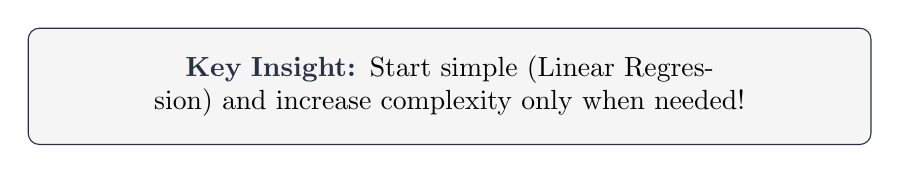
\begin{tikzpicture}
        \node[draw=databricksBlue, fill=databricksLightGray, rounded corners, text width=10cm, align=center, inner sep=10pt] {
            \textcolor{databricksBlue}{\textbf{Key Insight:}} Start simple (Linear Regression) and increase complexity only when needed!
        };
    \end{tikzpicture}
\end{frame}

% ============================================================
% Section: Model Selection Strategy
% ============================================================
\begin{frame}{Model Selection Strategy}
    \centering
    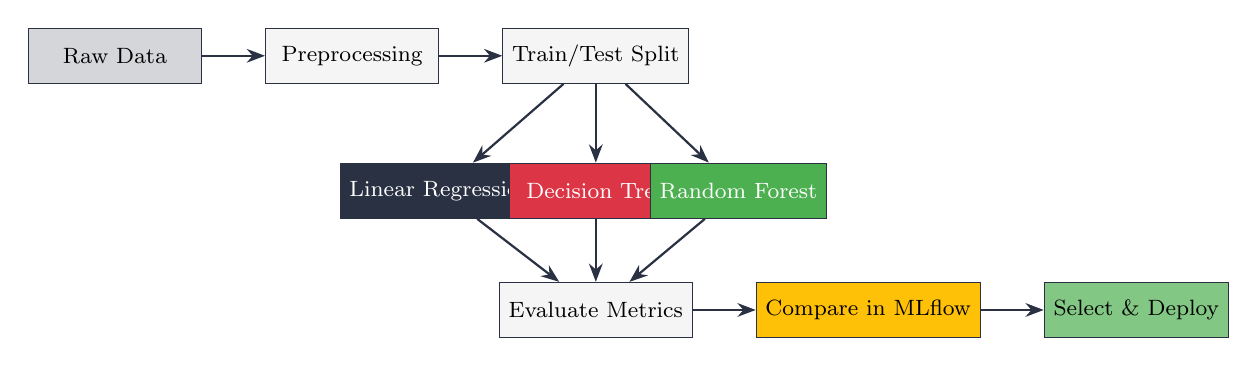
\begin{tikzpicture}[
        node distance=0.8cm,
        box/.style={rectangle, draw=databricksBlue, fill=databricksLightGray, minimum width=2.2cm, minimum height=0.7cm, align=center, font=\footnotesize},
        arrow/.style={-Stealth, thick, databricksBlue}
    ]
        % Flow nodes
        \node[box, fill=databricksBlue!20] (start) {Raw Data};
        \node[box, right=of start] (prep) {Preprocessing};
        \node[box, right=of prep] (split) {Train/Test Split};
        
        % Model nodes
        \node[box, fill=databricksBlue, text=white, below left=1cm and -0.5cm of split] (lr) {Linear Regression};
        \node[box, fill=databricksRed, text=white, below=1cm of split] (dt) {Decision Tree};
        \node[box, fill=databricksGreen, text=white, below right=1cm and -0.5cm of split] (rf) {Random Forest};
        
        % Evaluation nodes
        \node[box, below=0.8cm of dt] (eval) {Evaluate Metrics};
        \node[box, fill=databricksYellow, right=0.8cm of eval] (mlflow) {Compare in MLflow};
        \node[box, fill=databricksGreen!70, right=0.8cm of mlflow] (deploy) {Select \& Deploy};
        
        % Arrows
        \draw[arrow] (start) -- (prep);
        \draw[arrow] (prep) -- (split);
        \draw[arrow] (split) -- (lr);
        \draw[arrow] (split) -- (dt);
        \draw[arrow] (split) -- (rf);
        \draw[arrow] (lr) -- (eval);
        \draw[arrow] (dt) -- (eval);
        \draw[arrow] (rf) -- (eval);
        \draw[arrow] (eval) -- (mlflow);
        \draw[arrow] (mlflow) -- (deploy);
    \end{tikzpicture}
\end{frame}

% ============================================================
% Section: Hyperparameters
% ============================================================
\begin{frame}{What are Hyperparameters?}
    \begin{block}{Definition}
        Configuration settings that control the learning process — must be set \textbf{before} training begins.
    \end{block}
    
    \vspace{0.3cm}
    
    \centering
    \begin{tabular}{>{\columncolor{databricksBlue}\color{white}}l c c}
        \toprule
        \textbf{Aspect} & \textbf{Parameters} & \textbf{Hyperparameters} \\
        \midrule
        \rowcolor{databricksLightGray}
        Definition & Learned from data & Set before training \\
        Examples & Coefficients, weights & Learning rate, tree depth \\
        \rowcolor{databricksLightGray}
        How Set & Optimization algorithm & Manual or automated search \\
        Location & Inside the model & Outside the model \\
        \bottomrule
    \end{tabular}
\end{frame}

% ============================================================
% Section: Key Hyperparameters
% ============================================================
\begin{frame}{Key Hyperparameters by Model}
    \begin{columns}[T]
        \begin{column}{0.48\textwidth}
            \begin{block}{\textcolor{databricksBlue}{Decision Tree Regressor}}
                \small
                \begin{itemize}
                    \item[\textcolor{databricksBlue}{$\bullet$}] \texttt{max\_depth}
                    \begin{itemize}
                        \item[\textcolor{databricksRed}{$\triangleright$}] Maximum depth of tree
                        \item[\textcolor{databricksRed}{$\triangleright$}] Controls complexity
                    \end{itemize}
                    \vspace{0.2cm}
                    \item[\textcolor{databricksBlue}{$\bullet$}] \texttt{min\_samples\_split}
                    \begin{itemize}
                        \item[\textcolor{databricksRed}{$\triangleright$}] Min samples to split node
                    \end{itemize}
                    \vspace{0.2cm}
                    \item[\textcolor{databricksBlue}{$\bullet$}] \texttt{min\_samples\_leaf}
                    \begin{itemize}
                        \item[\textcolor{databricksRed}{$\triangleright$}] Min samples at leaf
                    \end{itemize}
                \end{itemize}
            \end{block}
        \end{column}
        
        \begin{column}{0.48\textwidth}
            \begin{block}{\textcolor{databricksRed}{Random Forest Regressor}}
                \small
                \begin{itemize}
                    \item[\textcolor{databricksBlue}{$\bullet$}] \texttt{n\_estimators}
                    \begin{itemize}
                        \item[\textcolor{databricksRed}{$\triangleright$}] Number of trees in forest
                    \end{itemize}
                    \vspace{0.2cm}
                    \item[\textcolor{databricksBlue}{$\bullet$}] \texttt{max\_depth}
                    \begin{itemize}
                        \item[\textcolor{databricksRed}{$\triangleright$}] Max depth of each tree
                    \end{itemize}
                    \vspace{0.2cm}
                    \item[\textcolor{databricksBlue}{$\bullet$}] \texttt{max\_features}
                    \begin{itemize}
                        \item[\textcolor{databricksRed}{$\triangleright$}] Features for best split
                    \end{itemize}
                \end{itemize}
            \end{block}
        \end{column}
    \end{columns}
\end{frame}

% ============================================================
% Section: Tuning Techniques
% ============================================================
\begin{frame}{Hyperparameter Tuning Techniques}
    \begin{columns}[T]
        \begin{column}{0.32\textwidth}
            
\begin{tikzpicture}
                \node[fill=databricksBlue, text=white, rounded corners, minimum width=3cm, minimum height=0.8cm, font=\bfseries] at (0,0) {Grid Search};
            \end{tikzpicture}
            \vspace{0.2cm}
            
            \footnotesize
            \textcolor{databricksBlue}{Exhaustive search} through specified parameter grid
            
            \vspace{0.2cm}
            \textcolor{databricksGreen}{$\checkmark$} Finds best combination
            
            \textcolor{databricksRed}{$\times$} Computationally expensive
        \end{column}
        
        \begin{column}{0.32\textwidth}
            
\begin{tikzpicture}
                \node[fill=databricksRed, text=white, rounded corners, minimum width=3cm, minimum height=0.8cm, font=\bfseries] at (0,0) {Random Search};
            \end{tikzpicture}
            \vspace{0.2cm}
            
            \footnotesize
            \textcolor{databricksBlue}{Samples random} combinations from distributions
            
            \vspace{0.2cm}
            \textcolor{databricksGreen}{$\checkmark$} More efficient
            
            \textcolor{databricksRed}{$\times$} May miss optimal
        \end{column}
        
        \begin{column}{0.32\textwidth}
            
\begin{tikzpicture}
                \node[fill=databricksGreen, text=white, rounded corners, minimum width=3cm, minimum height=0.8cm, font=\bfseries] at (0,0) {Bayesian Opt};
            \end{tikzpicture}
            \vspace{0.2cm}
            
            \footnotesize
            \textcolor{databricksBlue}{Probabilistic models} learn from evaluations
            
            \vspace{0.2cm}
            \textcolor{databricksGreen}{$\checkmark$} Most efficient
            
            \textcolor{databricksRed}{$\times$} Complex setup
        \end{column}
    \end{columns}
\end{frame}

% ============================================================
% Section: Grid Search Code
% ============================================================
\begin{frame}[fragile]{Grid Search Example}
\begin{lstlisting}[language=Python]
from sklearn.model_selection import GridSearchCV

param_grid = {
    'max_depth': [3, 5, 7, 10],
    'min_samples_split': [2, 5, 10]
}

grid_search = GridSearchCV(
    DecisionTreeRegressor(),
    param_grid,
    cv=5,  # 5-fold cross-validation
    scoring='r2'
)

grid_search.fit(X_train, y_train)
best_params = grid_search.best_params_
\end{lstlisting}
\end{frame}

% ============================================================
% Section: Feature Importance
% ============================================================
\begin{frame}{Understanding Feature Importance}
    \begin{block}{What is Feature Importance?}
        Quantifies how much each input feature contributes to the model's predictions.
    \end{block}
    
    \vspace{0.3cm}
    
    \begin{columns}[T]
        \begin{column}{0.48\textwidth}
            \textcolor{databricksBlue}{\textbf{Why It Matters:}}
            \begin{itemize}
                \item[\textcolor{databricksBlue}{$\bullet$}] \textbf{Understand the model}
                \begin{itemize}
                    \item[\textcolor{databricksRed}{$\triangleright$}] Know what drives predictions
                \end{itemize}
                \item[\textcolor{databricksBlue}{$\bullet$}] \textbf{Feature selection}
                \begin{itemize}
                    \item[\textcolor{databricksRed}{$\triangleright$}] Remove irrelevant features
                \end{itemize}
            \end{itemize}
        \end{column}
        
        \begin{column}{0.48\textwidth}
            \begin{itemize}
                \item[\textcolor{databricksBlue}{$\bullet$}] \textbf{Business insights}
                \begin{itemize}
                    \item[\textcolor{databricksRed}{$\triangleright$}] Identify key factors
                \end{itemize}
                \item[\textcolor{databricksBlue}{$\bullet$}] \textbf{Model debugging}
                \begin{itemize}
                    \item[\textcolor{databricksRed}{$\triangleright$}] Detect unexpected reliance
                \end{itemize}
            \end{itemize}
        \end{column}
    \end{columns}
\end{frame}

% ============================================================
% Section: Feature Importance Methods
% ============================================================
\begin{frame}{Methods to Calculate Feature Importance}
    \begin{columns}[T]
        \begin{column}{0.48\textwidth}
            \begin{block}{\textcolor{databricksBlue}{Coefficient Magnitude}}
                For Linear Regression:
                $$y = \beta_0 + \beta_1 x_1 + \ldots + \beta_n x_n$$
                
                Importance of feature $i$: $|\beta_i|$
            \end{block}
            
            \vspace{0.2cm}
            
            \begin{block}{\textcolor{databricksRed}{Gini Importance}}
                Mean Decrease in Impurity (MDI):
                $$\text{Imp}(f) = \sum_{t} \frac{n_t}{N} \cdot \Delta \text{impurity}_t$$
            \end{block}
        \end{column}
        
        \begin{column}{0.48\textwidth}
            \begin{block}{\textcolor{databricksGreen}{Permutation Importance}}
                Decrease in performance when feature shuffled:
                $$\text{Imp}(f) = \text{Score}_{orig} - \text{Score}_{perm}$$
            \end{block}
            
            \vspace{0.2cm}
            
            \footnotesize
            \textcolor{databricksBlue}{\textbf{Model-agnostic:}} Works with any model
            
            \textcolor{databricksGreen}{\textbf{Robust:}} Based on actual predictions
        \end{column}
    \end{columns}
\end{frame}

% ============================================================
% Section: Spark ML Pipelines
% ============================================================
\begin{frame}{What is a Spark ML Pipeline?}
    \begin{block}{Definition}
        A sequence of stages that transform data and train models — chains transformers and estimators into a single workflow.
    \end{block}
    
    \vspace{0.3cm}
    
    \centering
    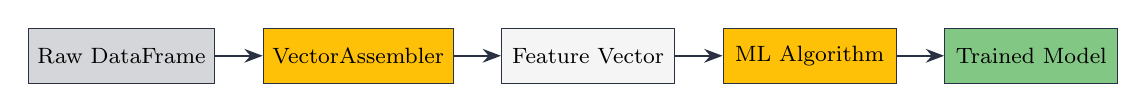
\begin{tikzpicture}[
        node distance=0.6cm,
        box/.style={rectangle, draw=databricksBlue, fill=databricksLightGray, minimum width=2.2cm, minimum height=0.7cm, align=center, font=\footnotesize},
        arrow/.style={-Stealth, thick, databricksBlue}
    ]
        \node[box, fill=databricksBlue!20] (raw) {Raw DataFrame};
        \node[box, fill=databricksYellow, right=of raw] (va) {VectorAssembler};
        \node[box, right=of va] (vec) {Feature Vector};
        \node[box, fill=databricksYellow, right=of vec] (ml) {ML Algorithm};
        \node[box, fill=databricksGreen!70, right=of ml] (model) {Trained Model};
        
        \draw[arrow] (raw) -- (va);
        \draw[arrow] (va) -- (vec);
        \draw[arrow] (vec) -- (ml);
        \draw[arrow] (ml) -- (model);
    \end{tikzpicture}
    
    \vspace{0.4cm}
    
    \begin{columns}[T]
        \begin{column}{0.32\textwidth}
            \centering
            \textcolor{databricksBlue}{\textbf{Reproducibility}}\\
            \footnotesize Same transformations consistently
        \end{column}
        \begin{column}{0.32\textwidth}
            \centering
            \textcolor{databricksRed}{\textbf{Simplicity}}\\
            \footnotesize Complex workflows as single objects
        \end{column}
        \begin{column}{0.32\textwidth}
            \centering
            \textcolor{databricksGreen}{\textbf{No Data Leakage}}\\
            \footnotesize Transformations fit only on train
        \end{column}
    \end{columns}
\end{frame}

% ============================================================
% Section: Pipeline Components
% ============================================================
\begin{frame}{Pipeline Components}
    \begin{columns}[T]
        \begin{column}{0.48\textwidth}
            \begin{block}{\textcolor{databricksBlue}{Transformers}}
                Convert one DataFrame into another (no learning)
            \end{block}
            
            \footnotesize
            \begin{tabular}{l l}
                \texttt{VectorAssembler} & Combine cols → vector \\
                \texttt{StringIndexer} & Strings → numeric \\
                \texttt{StandardScaler} & Mean=0, Std=1 \\
                \texttt{OneHotEncoder} & One-hot vectors \\
            \end{tabular}
        \end{column}
        
        \begin{column}{0.48\textwidth}
            \begin{block}{\textcolor{databricksRed}{Estimators}}
                Learn from data, produce a Model
            \end{block}
            
            \footnotesize
            \begin{tabular}{l l}
                \texttt{LinearRegression} & → LRModel \\
                \texttt{DecisionTreeRegressor} & → DTModel \\
                \texttt{RandomForestRegressor} & → RFModel \\
            \end{tabular}
        \end{column}
    \end{columns}
    
    \vspace{0.4cm}
    
    \centering
    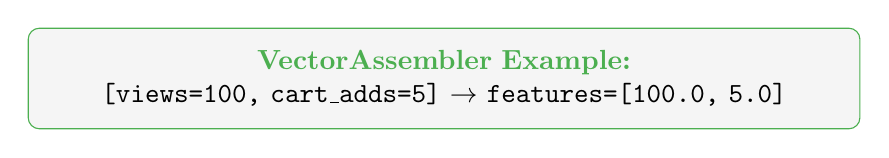
\begin{tikzpicture}
        \node[draw=databricksGreen, fill=databricksLightGray, rounded corners, text width=10cm, align=center, inner sep=8pt] {
            \textcolor{databricksGreen}{\textbf{VectorAssembler Example:}}\\
            \texttt{[views=100, cart\_adds=5]} $\rightarrow$ \texttt{features=[100.0, 5.0]}
        };
    \end{tikzpicture}
\end{frame}

% ============================================================
% Section: Pipeline Code
% ============================================================
\begin{frame}[fragile]{Building a Spark ML Pipeline}
\begin{lstlisting}[language=Python, basicstyle=\ttfamily\scriptsize]
from pyspark.ml import Pipeline
from pyspark.ml.feature import VectorAssembler
from pyspark.ml.regression import LinearRegression as SparkLR

# Stage 1: Combine features into vector
assembler = VectorAssembler(
    inputCols=["views", "cart_adds"],
    outputCol="features"
)

# Stage 2: Linear Regression
lr = SparkLR(featuresCol="features", labelCol="purchases")

# Create and fit pipeline
pipeline = Pipeline(stages=[assembler, lr])
model = pipeline.fit(train_df)

# Make predictions
predictions = model.transform(test_df)
\end{lstlisting}
\end{frame}

% ============================================================
% Section: MLflow Integration
% ============================================================
\begin{frame}{MLflow Integration for Model Tracking}
    \begin{columns}[T]
        \begin{column}{0.5\textwidth}
            \textcolor{databricksBlue}{\textbf{MLflow Provides:}}
            \begin{itemize}
                \item[\textcolor{databricksBlue}{$\bullet$}] \textbf{Experiment Tracking}
                \begin{itemize}
                    \item[\textcolor{databricksRed}{$\triangleright$}] Log params, metrics, artifacts
                \end{itemize}
                \item[\textcolor{databricksBlue}{$\bullet$}] \textbf{Model Registry}
                \begin{itemize}
                    \item[\textcolor{databricksRed}{$\triangleright$}] Version and manage models
                \end{itemize}
                \item[\textcolor{databricksBlue}{$\bullet$}] \textbf{Model Deployment}
                \begin{itemize}
                    \item[\textcolor{databricksRed}{$\triangleright$}] Deploy as REST APIs
                \end{itemize}
            \end{itemize}
        \end{column}
        
        \begin{column}{0.5\textwidth}
            \centering
            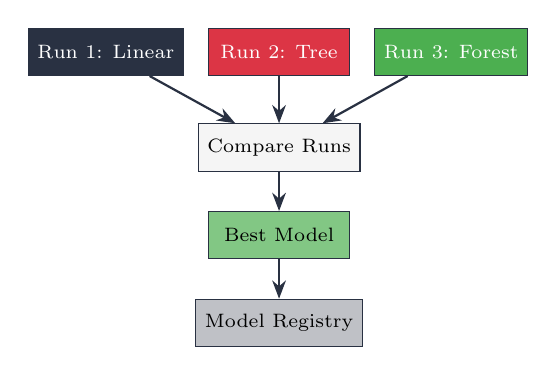
\begin{tikzpicture}[
                node distance=0.5cm,
                box/.style={rectangle, draw=databricksBlue, fill=databricksLightGray, minimum width=1.8cm, minimum height=0.6cm, align=center, font=\scriptsize},
                arrow/.style={-Stealth, thick, databricksBlue}
            ]
                \node[box, fill=databricksBlue, text=white] (r1) {Run 1: Linear};
                \node[box, fill=databricksRed, text=white, right=0.3cm of r1] (r2) {Run 2: Tree};
                \node[box, fill=databricksGreen, text=white, right=0.3cm of r2] (r3) {Run 3: Forest};
                
                \node[box, below=0.6cm of r2] (compare) {Compare Runs};
                \node[box, fill=databricksGreen!70, below=0.5cm of compare] (best) {Best Model};
                \node[box, fill=databricksBlue!30, below=0.5cm of best] (reg) {Model Registry};
                
                \draw[arrow] (r1) -- (compare);
                \draw[arrow] (r2) -- (compare);
                \draw[arrow] (r3) -- (compare);
                \draw[arrow] (compare) -- (best);
                \draw[arrow] (best) -- (reg);
            \end{tikzpicture}
        \end{column}
    \end{columns}
\end{frame}

% ============================================================
% Section: MLflow Functions
% ============================================================
\begin{frame}{Key MLflow Functions}
    \centering
    \small
    \begin{tabular}{>{\columncolor{databricksBlue}\color{white}}l l l}
        \toprule
        \textbf{Function} & \textbf{Purpose} & \textbf{Example} \\
        \midrule
        \rowcolor{databricksLightGray}
        \texttt{start\_run()} & Start a new run & \texttt{with mlflow.start\_run():} \\
        \texttt{log\_param()} & Log a parameter & \texttt{mlflow.log\_param("depth", 5)} \\
        \rowcolor{databricksLightGray}
        \texttt{log\_metric()} & Log a metric & \texttt{mlflow.log\_metric("r2", 0.85)} \\
        \texttt{log\_artifact()} & Log a file & \texttt{mlflow.log\_artifact("plot.png")} \\
        \rowcolor{databricksLightGray}
        \texttt{sklearn.log\_model()} & Log sklearn model & \texttt{mlflow.sklearn.log\_model(...)} \\
        \bottomrule
    \end{tabular}
    
    \vspace{0.5cm}
    
    
\begin{tikzpicture}
        \node[draw=databricksBlue, fill=databricksLightGray, rounded corners, text width=10cm, align=center, inner sep=8pt] {
            \textcolor{databricksBlue}{\textbf{Tip:}} Use \texttt{with mlflow.start\_run():} for automatic run closure!
        };
    \end{tikzpicture}
\end{frame}

% ============================================================
% Section: Training Loop Code
% ============================================================
\begin{frame}[fragile]{Training Loop with MLflow}
\begin{lstlisting}[language=Python, basicstyle=\ttfamily\scriptsize]
models = {
    "linear": LinearRegression(),
    "decision_tree": DecisionTreeRegressor(max_depth=5),
    "random_forest": RandomForestRegressor(n_estimators=100)
}

for name, model in models.items():
    with mlflow.start_run(run_name=f"{name}_model"):
        # Log model type
        mlflow.log_param("model_type", name)
        
        # Train and evaluate
        model.fit(X_train, y_train)
        score = model.score(X_test, y_test)
        
        # Log metrics and model
        mlflow.log_metric("r2_score", score)
        mlflow.sklearn.log_model(model, "model")
        
        print(f"{name}: R2 = {score:.4f}")
\end{lstlisting}
\end{frame}

% ============================================================
% Section: R² Metric
% ============================================================
\begin{frame}{Understanding R² (Coefficient of Determination)}
    \begin{block}{Formula}
        $$R^2 = 1 - \frac{SS_{res}}{SS_{tot}} = 1 - \frac{\sum_{i=1}^{n} (y_i - \hat{y}_i)^2}{\sum_{i=1}^{n} (y_i - \bar{y})^2}$$
    \end{block}
    
    \vspace{0.3cm}
    
    \begin{columns}[T]
        \begin{column}{0.48\textwidth}
            \textcolor{databricksBlue}{\textbf{Calculation Steps:}}
            \begin{enumerate}
                \item Calculate mean: $\bar{y} = \frac{1}{n}\sum y_i$
                \item Total variance: $SS_{tot}$
                \item Residual variance: $SS_{res}$
                \item Compute R²
            \end{enumerate}
        \end{column}
        
        \begin{column}{0.48\textwidth}
            \textcolor{databricksRed}{\textbf{Interpretation:}}
            \begin{itemize}
                \item[\textcolor{databricksGreen}{$\bullet$}] $R^2 = 1.0$: Perfect predictions
                \item[\textcolor{databricksYellow}{$\bullet$}] $R^2 = 0.0$: Predicts mean only
                \item[\textcolor{databricksRed}{$\bullet$}] $R^2 < 0$: Worse than mean
            \end{itemize}
        \end{column}
    \end{columns}
\end{frame}

% ============================================================
% Section: Other Metrics
% ============================================================
\begin{frame}{Regression Metrics Comparison}
    \centering
    \begin{tabular}{>{\columncolor{databricksBlue}\color{white}}l c c}
        \toprule
        \textbf{Metric} & \textbf{Formula} & \textbf{Use Case} \\
        \midrule
        \rowcolor{databricksLightGray}
        MSE & $\frac{1}{n} \sum (y_i - \hat{y}_i)^2$ & Penalizes large errors \\
        RMSE & $\sqrt{\frac{1}{n} \sum (y_i - \hat{y}_i)^2}$ & Same units as target \\
        \rowcolor{databricksLightGray}
        MAE & $\frac{1}{n} \sum |y_i - \hat{y}_i|$ & Robust to outliers \\
        MAPE & $\frac{100}{n} \sum \left|\frac{y_i - \hat{y}_i}{y_i}\right|$ & Percentage error \\
        \bottomrule
    \end{tabular}
    
    \vspace{0.5cm}
    
    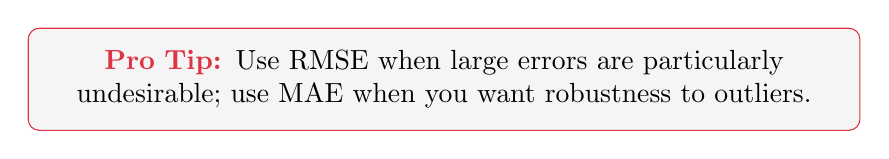
\begin{tikzpicture}
        \node[draw=databricksRed, fill=databricksLightGray, rounded corners, text width=10cm, align=center, inner sep=8pt] {
            \textcolor{databricksRed}{\textbf{Pro Tip:}} Use RMSE when large errors are particularly undesirable; use MAE when you want robustness to outliers.
        };
    \end{tikzpicture}
\end{frame}

% ============================================================
% Section: Model Comparison Example
% ============================================================
\begin{frame}{Model Comparison Example}
    \centering
    \begin{tabular}{>{\columncolor{databricksBlue}\color{white}}l c c c}
        \toprule
        \textbf{Model} & \textbf{R² Score} & \textbf{Training Time} & \textbf{Interpretability} \\
        \midrule
        \rowcolor{databricksLightGray}
        Linear Regression & 0.7234 & 0.5s & \textcolor{databricksGreen}{High} \\
        Decision Tree & 0.7856 & 1.2s & \textcolor{databricksYellow}{Medium} \\
        \rowcolor{databricksLightGray}
        Random Forest & \textcolor{databricksGreen}{\textbf{0.8421}} & 8.5s & \textcolor{databricksRed}{Low} \\
        \bottomrule
    \end{tabular}
    
    \vspace{0.4cm}
    
    \begin{columns}[T]
        \begin{column}{0.48\textwidth}
            \textcolor{databricksBlue}{\textbf{Selection Factors:}}
            \begin{itemize}
                \item[\textcolor{databricksBlue}{$\bullet$}] Performance (R² score)
                \item[\textcolor{databricksBlue}{$\bullet$}] Training speed
                \item[\textcolor{databricksBlue}{$\bullet$}] Interpretability needs
                \item[\textcolor{databricksBlue}{$\bullet$}] Business requirements
            \end{itemize}
        \end{column}
        
        \begin{column}{0.48\textwidth}
            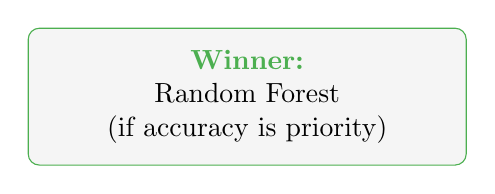
\begin{tikzpicture}
                \node[draw=databricksGreen, fill=databricksLightGray, rounded corners, text width=5cm, align=center, inner sep=8pt] {
                    \textcolor{databricksGreen}{\textbf{Winner:}}\\
                    Random Forest\\
                    (if accuracy is priority)
                };
            \end{tikzpicture}
        \end{column}
    \end{columns}
\end{frame}

% ============================================================
% Section: Best Practices
% ============================================================
\begin{frame}{Best Practices}
    \begin{columns}[T]
        \begin{column}{0.48\textwidth}
            \textcolor{databricksBlue}{\textbf{Data Preparation}}
            \begin{itemize}
                \item[\textcolor{databricksBlue}{$\bullet$}] Split data before preprocessing
                \item[\textcolor{databricksBlue}{$\bullet$}] Use cross-validation
                \item[\textcolor{databricksBlue}{$\bullet$}] Handle missing values consistently
            \end{itemize}
            
            \vspace{0.3cm}
            
            \textcolor{databricksRed}{\textbf{Model Training}}
            \begin{itemize}
                \item[\textcolor{databricksRed}{$\bullet$}] Start simple before complex
                \item[\textcolor{databricksRed}{$\bullet$}] Use consistent random seeds
                \item[\textcolor{databricksRed}{$\bullet$}] Log everything with MLflow
            \end{itemize}
        \end{column}
        
        \begin{column}{0.48\textwidth}
            \textcolor{databricksGreen}{\textbf{Feature Engineering}}
            \begin{itemize}
                \item[\textcolor{databricksGreen}{$\bullet$}] Use domain knowledge
                \item[\textcolor{databricksGreen}{$\bullet$}] Remove correlated features
                \item[\textcolor{databricksGreen}{$\bullet$}] Scale when needed
            \end{itemize}
            
            \vspace{0.3cm}
            
            \textcolor{databricksOrange}{\textbf{Pipeline Design}}
            \begin{itemize}
                \item[\textcolor{databricksOrange}{$\bullet$}] Include all preprocessing
                \item[\textcolor{databricksOrange}{$\bullet$}] Save fitted pipelines
                \item[\textcolor{databricksOrange}{$\bullet$}] Version your pipelines
            \end{itemize}
        \end{column}
    \end{columns}
\end{frame}

% ============================================================
% Section: Model Selection Guide
% ============================================================
\begin{frame}{Quick Reference: Model Selection Guide}
    \centering
    \begin{tabular}{>{\columncolor{databricksBlue}\color{white}}l l}
        \toprule
        \textbf{Situation} & \textbf{Recommended Model} \\
        \midrule
        \rowcolor{databricksLightGray}
        Need interpretability & Linear Regression \\
        Non-linear relationships & Decision Tree / Random Forest \\
        \rowcolor{databricksLightGray}
        High accuracy required & Random Forest (with tuning) \\
        Large distributed data & Spark ML Pipeline \\
        \rowcolor{databricksLightGray}
        Quick baseline & Linear Regression \\
        \bottomrule
    \end{tabular}
    
    \vspace{0.5cm}
    
    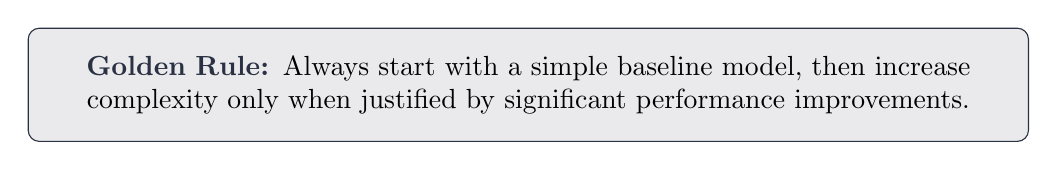
\begin{tikzpicture}
        \node[draw=databricksBlue, fill=databricksBlue!10, rounded corners, text width=12cm, align=center, inner sep=10pt] {
            \textcolor{databricksBlue}{\textbf{Golden Rule:}} Always start with a simple baseline model, then increase complexity only when justified by significant performance improvements.
        };
    \end{tikzpicture}
\end{frame}

% ============================================================
% Section: Complete Workflow
% ============================================================
\begin{frame}{Complete Workflow Summary}
    \centering
    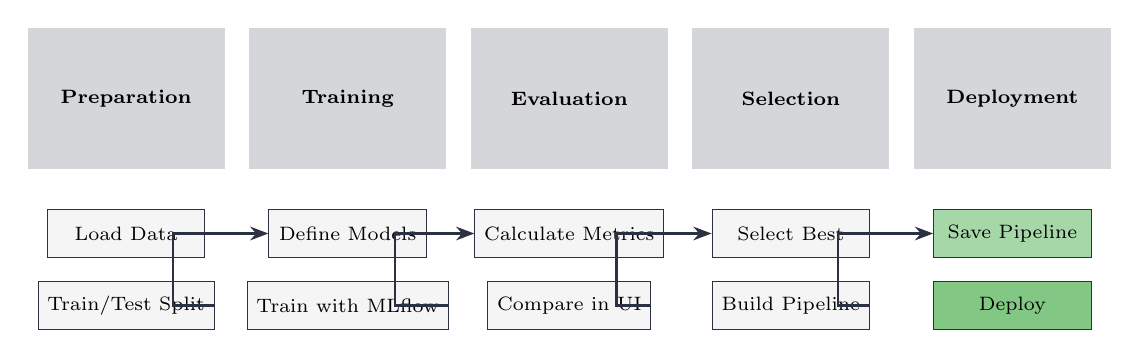
\begin{tikzpicture}[
        node distance=0.4cm,
        box/.style={rectangle, draw=databricksBlue, fill=databricksLightGray, minimum width=2cm, minimum height=0.6cm, align=center, font=\scriptsize},
        phase/.style={rectangle, draw=none, fill=databricksBlue!20, minimum width=2.5cm, minimum height=1.8cm, align=center, font=\scriptsize\bfseries},
        arrow/.style={-Stealth, thick, databricksBlue}
    ]
        % Phases
        \node[phase] (p1) {Preparation};
        \node[phase, right=0.3cm of p1] (p2) {Training};
        \node[phase, right=0.3cm of p2] (p3) {Evaluation};
        \node[phase, right=0.3cm of p3] (p4) {Selection};
        \node[phase, right=0.3cm of p4] (p5) {Deployment};
        
        % Steps
        \node[box, below=0.5cm of p1] (s1) {Load Data};
        \node[box, below=0.3cm of s1] (s2) {Train/Test Split};
        
        \node[box, below=0.5cm of p2] (s3) {Define Models};
        \node[box, below=0.3cm of s3] (s4) {Train with MLflow};
        
        \node[box, below=0.5cm of p3] (s5) {Calculate Metrics};
        \node[box, below=0.3cm of s5] (s6) {Compare in UI};
        
        \node[box, below=0.5cm of p4] (s7) {Select Best};
        \node[box, below=0.3cm of s7] (s8) {Build Pipeline};
        
        \node[box, fill=databricksGreen!50, below=0.5cm of p5] (s9) {Save Pipeline};
        \node[box, fill=databricksGreen!70, below=0.3cm of s9] (s10) {Deploy};
        
        % Arrows
        \draw[arrow] (s2) -- ++(0.6,0) |- (s3);
        \draw[arrow] (s4) -- ++(0.6,0) |- (s5);
        \draw[arrow] (s6) -- ++(0.6,0) |- (s7);
        \draw[arrow] (s8) -- ++(0.6,0) |- (s9);
    \end{tikzpicture}
\end{frame}

% ============================================================
% Section: Key Takeaways
% ============================================================
\begin{frame}{Key Takeaways}
    \begin{columns}[T]
        \begin{column}{0.48\textwidth}
            
\begin{tikzpicture}
                \node[fill=databricksBlue, text=white, rounded corners, minimum width=4cm, minimum height=0.7cm, font=\footnotesize\bfseries] at (0,0) {1. Multiple Models};
            \end{tikzpicture}
            \footnotesize No single model works best for all problems
            
            \vspace{0.3cm}
            
            
\begin{tikzpicture}
                \node[fill=databricksRed, text=white, rounded corners, minimum width=4cm, minimum height=0.7cm, font=\footnotesize\bfseries] at (0,0) {2. MLflow Tracking};
            \end{tikzpicture}
            \footnotesize Enables reproducibility and comparison
            
            \vspace{0.3cm}
            
            
\begin{tikzpicture}
                \node[fill=databricksGreen, text=white, rounded corners, minimum width=4cm, minimum height=0.7cm, font=\footnotesize\bfseries] at (0,0) {3. Spark ML Pipelines};
            \end{tikzpicture}
            \footnotesize Chain transformations for production
        \end{column}
        
        \begin{column}{0.48\textwidth}
            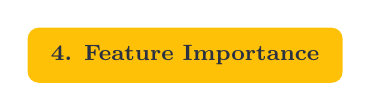
\begin{tikzpicture}
                \node[fill=databricksYellow, text=databricksBlue, rounded corners, minimum width=4cm, minimum height=0.7cm, font=\footnotesize\bfseries] at (0,0) {4. Feature Importance};
            \end{tikzpicture}
            \footnotesize Understand what features matter
            
            \vspace{0.3cm}
            
            
\begin{tikzpicture}
                \node[fill=databricksPurple, text=white, rounded corners, minimum width=4cm, minimum height=0.7cm, font=\footnotesize\bfseries] at (0,0) {5. Hyperparameters};
            \end{tikzpicture}
            \footnotesize \texttt{max\_depth} and \texttt{n\_estimators} control complexity
        \end{column}
    \end{columns}
\end{frame}

% ============================================================
% Thank You Slide
% ============================================================
{
\setbeamertemplate{footline}{}
\begin{frame}
\begin{tikzpicture}[remember picture, overlay]
    % Background
    \fill[databricksBlue] (current page.south west) rectangle (current page.north east);
    
    % Decorative circles
    \fill[databricksRed, opacity=0.3] (current page.north east) ++(-3,-2) circle (3cm);
    \fill[databricksGreen, opacity=0.2] (current page.south west) ++(2,2) circle (3cm);
    \fill[databricksYellow, opacity=0.2] (current page.west) ++(1,0) circle (2cm);
    
    % Content
    \node[anchor=center, text width=0.8\paperwidth, align=center] at (current page.center) {
        {\Huge\bfseries\textcolor{databricksWhite}{Thank You!}}\\[0.5cm]
        {\large\textcolor{databricksYellow}{Day 13: Model Comparison \& Feature Engineering}}\\[0.8cm]
        {\normalsize\textcolor{databricksLightGray}{Connect with me:}}\\[0.3cm]
        {\small\textcolor{databricksWhite}{
            \href{https://www.linkedin.com/in/yashkavaiya}{LinkedIn: Yash Kavaiya} \\[0.2cm]
            \href{https://www.linkedin.com/company/genai-guru}{Gen AI Guru} \\[0.2cm]
            \href{https://easy-ai-labs.lovable.app/}{Easy AI Labs}
        }}
    };
    
    % Bottom decoration
    \fill[databricksYellow] (current page.south west) rectangle ++(0.33\paperwidth, 0.15);
    \fill[databricksRed] (current page.south west) ++(0.33\paperwidth,0) rectangle ++(0.34\paperwidth, 0.15);
    \fill[databricksGreen] (current page.south west) ++(0.67\paperwidth,0) rectangle ++(0.33\paperwidth, 0.15);
\end{tikzpicture}
\end{frame}
}

\end{document}
